\chapter{Datenanalyse} \label{sec:datenAnalyse}
Dieser abschnitt hat 2 ziele 1. eine gute auswahl an code basen finden, die wir sowohl für unsere algorithmus anpassungen als auch für die evaluation am ende verwenden können.
2. wollen wir die Struktur von Softwareprojekten näher untersuchen, um zu verstehen, wie sie aufgebaut sind und welche Eigenschaften sie haben.

wie gesagt wir wollen die Struktur näher bestimmen. Wie definiert ist die struktur immer eine baumstruktur. 
Wir interessieren uns dabei für zwei spezielle Aspekte. 
1. Die Hierarchie-Tiefe, also wie tief die Verschachtelung der Knoten ist. 
%warum wollen wir baum tiefe?
Zeigt uns worauf wir uns bei der Visualierung fokussieren müssen, entwerder darauf die order schachtelung zu optimieren oder darauf die geschwister zu optimieren.
%wie messen wir dann?

2. Die Anzahl der Kinder-Knoten eines Knotens, also wie viele geschwister knoten ein Knoten hat. Dieser Wert ist wichtig, da beim squarify algirhtmus, so wie wir in implementieren und anpassen, die laufzeit in jedem schritt von der Anzahl der Kinder-Knoten abhängt.
Interessant ist das, weil wir in jedem neuen squarify schritt des algotihmus zb. eine sortierung der Kinder anlegen. Außerdem ist es interessant, weil wir in jedem algotihmus schritt immer nur alle geschister betrachten

3. Die Anzahl der Knoten insgesamt, also wie viele DAteien in dem Projekt enthalten sind. Dieser Wert ist wichtig, da die Laufzeit des Algorithmus von der Anzahl der Knoten abhängt.
Tivial. Das ist wichtig, weil das die laufzeit des algorithmus beeinflusst und natürlich auch die Visualisierung selbst.
knoten sind dateien plus ordner. es kommt uns also gar nicht nur auf die order an.



\section{Auswahl der Projekte} \label{sec:auswahlDerProjekte}
Als Quelle werden wir GitHub verwenden, da es eine große Anzahl an Open-Source-Projekten bietet und die Daten leicht zugänglich sind.
Wir gehen nicht davon aus, dass es einen signifikanten Unterschied zwischen Open-Source und Closed-Source Projekten gibt \cite{closedVsOpenSource, closedVsOpenSource2}, weshalb wir nur auf open source zugreifen 
Wir probieren möglich breit gefächert Projekte zu betrachten, um ein möglichst breites Spektrum an Softwareprojekten abzudecken. 
Das Ziel bei der Auswahl der Projekte ist es, eine möglichst diverse Auswahl an Projekten zu haben, um später eine Aussage über die Struktur von Softwareprojekten im Allgemeinen treffen zu können und nicht nur über die Stuktur der meisten Softwareprojekte. Wir könnten einfach zufällige Projekte von Github auswählen, aber das würde vermutlich zu einer Verzerrung führen und eher kleinere und unbekannte Projekte auswählen.
Deshalb suchen wir nach Kriterien, die einen Einfluss auf die Struktur von Softwareprojekten haben könnten. 

da es keine quellen gibt, die eine solche Auswahl an Kriterien vorgeben, können wir nur vermutungen anstellen und diese im nachhinein anhand der Daten überprüfen, können aber nicht sicher garantieren, dass wir wirklich alle relevanten Kriterien berücksichtigt haben. aber das ist ja auch keine arbeit über die selektion von Projekten, deshalb geben wir uns damit zufrieden.
Zur identifikation von relevanten Kriterien richten wir uns nach den informationen, die die GitHub API uns zur verfügung stellt. Es gibt eine Vielzahl an Metainformationen. 

Wir wählen initial 50 repositories aus. diese repositories wählen wir aus anhand der folgenden Kriterien. Dann überprüfen wir, ob die Kriterien tatsächlich einen Einfluss auf die Struktur der Projekte haben.

\subsection*{Programmiersprache} Wir werden Projekte in verschiedenen Programmiersprachen betrachten, da die Struktur von Softwareprojekten in verschiedenen Programmiersprachen stark unterschiedlich sein kann - hier fehlt noch ein beweis - ist da überhaupt so? wenn nicht kann man das auch weglassen. Wir wählen die Programmiersprachen nach ihrer Popularität und Paradigma aus. 
    \begin{itemize}
        \item \textbf{Python:} Die zweit populärste Sprache \cite{software_state_2022} mit dynamischer Typisierung, sowohl imperativem als auch objektorientiertem Paradigma. 
        \item \textbf{JavaScript:} die populärste Sprache \cite{software_state_2022} mit dynamischer Typisierung. Die Struktur von JavaScript-Projekten ist besonders geprägt durch Frameworks.
        \item \textbf{Java:} Die dritt populärste Sprache \cite{software_state_2022} mit statischer Typisierung und objektorientiertem Paradigma. Java-Projekte sind oft sehr strukturiert und folgen bestimmten Konventionen.
        \item \textbf{C:} Eine der ältesten Programmiersprachen, die immer noch weit verbreitet ist (Platz 9 \cite{software_state_2022}). C-Projekte sind oft sehr nah an der Hardware und haben eine andere Struktur als Projekte in höheren Programmiersprachen.
        \item \textbf{Shell:} Eine Skriptsprache (Platz 8 \cite{software_state_2022}), die oft für Automatisierung und Systemadministration verwendet wird.
    \end{itemize}
   kleiner spoiler: Wir werden sehen, dass die Programmiersprache tatsächlich einen Einfluss auf die Struktur von Softwareprojekten hat.


\subsection*{Projektgröße} Die Projektgröße ist offensichlich der Wichtigste Faktor für die STruktur eines Projekts. Wir gehen davon aus, dass Große Projekte auch dann größere Strukturen (also mehr knoten) haben (stimmt nicht zwingen - wie im folgenden ABschnit \ref{sec:auswahlDerProjekteImDetail} gezeigt wird) Github bietet leider nur die möglichkeit nach größe und nicht nach Anzahl der Dateien zu filtern, was uns eigentich interessieren würde. 
kleiner spoiler: Wir werden sehen, dass die Programmiersprache tatsächlich einen Einfluss auf die Struktur von Softwareprojekten hat.

\subsection*{Ungenutzte Kategorien}
Man könnte denken, dass auch andere Kategorien wie die Anzahl der Sterne oder die Anzahl der Mitwirkenden eines Projekts einen Einfluss auf die Struktur eines Projekts haben. Wir hatten auch diese vermutung und haben dies nachgeprüft. Um fragen zu vermeiden zeigen wir hier auch die ergebnisse, die gezeigt haben dass diese Kategorien keinen Einfluss haben und wir sie deshalb verworfen haben.

1. Wir gingen davon aus, dass die Popularität eines Projekts einen Einfluss auf die Qualität eines Projekts hat. Je Popularitärer ein Projekt ist, desto "besser" muss es sein, desto besser muss ja auch die Qualität sein. Und wir gehen davon aus, dass die Qualität eines Projekts einen Einfluss auf die Struktur des Projekts hat. Allerdings deutet eine Studie an, dass Popularität nicht in Korrelation mit Software Qualität steht \cite{popAndQuality}. Außerdem sind die meisten Projekte die auf GitHub viele Sterne haben eher Sammlungen von Bücher, Kursen oder anderen Ressourcen und nicht wirklich Softwareprojekte \cite{evanli_github-ranking_2025}, weshalb wir uns entschieden haben, die Popularität nicht als Kriterium zu verwenden, auch wenn es auf den ersten Blick sinnvoll erscheinen mag.

2. Eine größere Anzahl an Mitwirkenden, mehr Änderungen und generell mehr aufmerksamkeit. 
Es gibt paper, die sagen, dass unterschiedlichen Anzahlen an Mitwirkenden hat einen Einfluss auf die Struktur und Qualität des Codes haben kann \cite{numDevs}. Wir werden nur Projekte bereits ab einer Anzahl von 2 Mitwirkenden betrachten, da Projekte mit nur einem Mitwirkenden oft nicht wirklich repräsentativ für die Struktur von Softwareprojekten sind. 
Wir überprufen, ob die Anzahl der Mitwirkenden einen Einfluss auf die Struktur - konkret die Hierarchie-Tiefe und die Anzahl der Kinder-Knoten - hat.

\begin{figure}
    \centering
    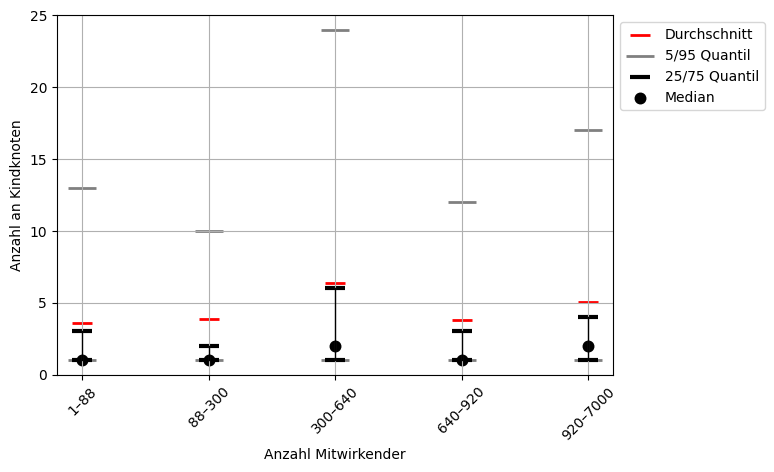
\includegraphics[width=0.8\textwidth]{images/datenanalyse/mitwirkendeVsKindknoten.png}
    \caption{Die Anzahl der Mitwirkenden auf der x-Achse hat keinen erkennbaren Einfluss auf die Anzahl der Kinder-Knoten eines Knotens.}
    \label{fig:mitwirkendeVsKindknoten}
\end{figure}

\begin{figure}
    \centering
    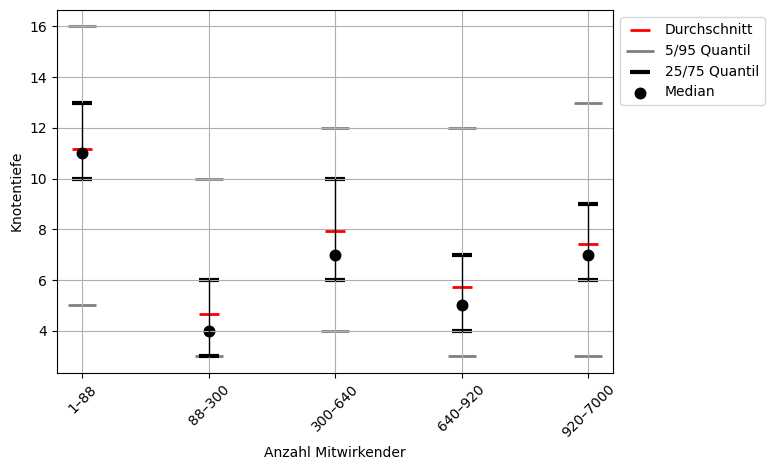
\includegraphics[width=0.8\textwidth]{images/datenanalyse/mitwirkendeVsTiefe.png}
    \caption{Die Anzahl der Mitwirkenden auf der x-Achse hat keinen erkennbaren Einfluss auf die Hierarchie-Tiefe eines Knotens.}
    \label{fig:mitwirkendeVsTiefe}
\end{figure}

\subsection{Die Auswahl der Projekte im Detail} \label{sec:auswahlDerProjekteImDetail}
So wir wissen jetzt, dass wir nur auf sprache und größe achten wollen. wir haben 5 verschiedene bekannte sprachen und verschiedene größen. Wir nehmen eine gute anzahl an Projekten, so dass jede kombi repräsentiert ist, aber trotzdem nur so viele wie wir rechnerisch handlen können. 
In Abbildung \ref{fig:repoGroesseVerteilungUnfiltered} haben wir die Verteilung der Projektgrößen von 2500 zufällig ausgewählten GitHub-Repositories dargestellt. Es ist zu erkennen, dass es deutlich mehr kleinere Projekte gibt. (Zur Größen einordung: das REact repository, was als ein sehr großes Projekt gilt, hat eine Größe von ca.  einem Gigabyte)
Wir wollen die Größe von 98 Prozent aller Repositories abdekcen. Wir haben uns für diesen Wert entschieden, da wir eine sehr gute Abdeckung auch großer Projekte haben wollen, aber trotzdem auch nicht zu viele Projekte generell haben wollen. Außerdem ab dieser Größe wird es wahrscheinlich generell sehr schwer sinnvoll zu visualisieren bereits das React Repo kann mit 1GB teilweise unübersichlich werden, nicht weil der algorithmus oder die visualisierung schlcht ist sondern weil es einfach zu viele Dateien werden irgendwann. %beispiel für react visualisierung

\begin{figure}
    \centering
    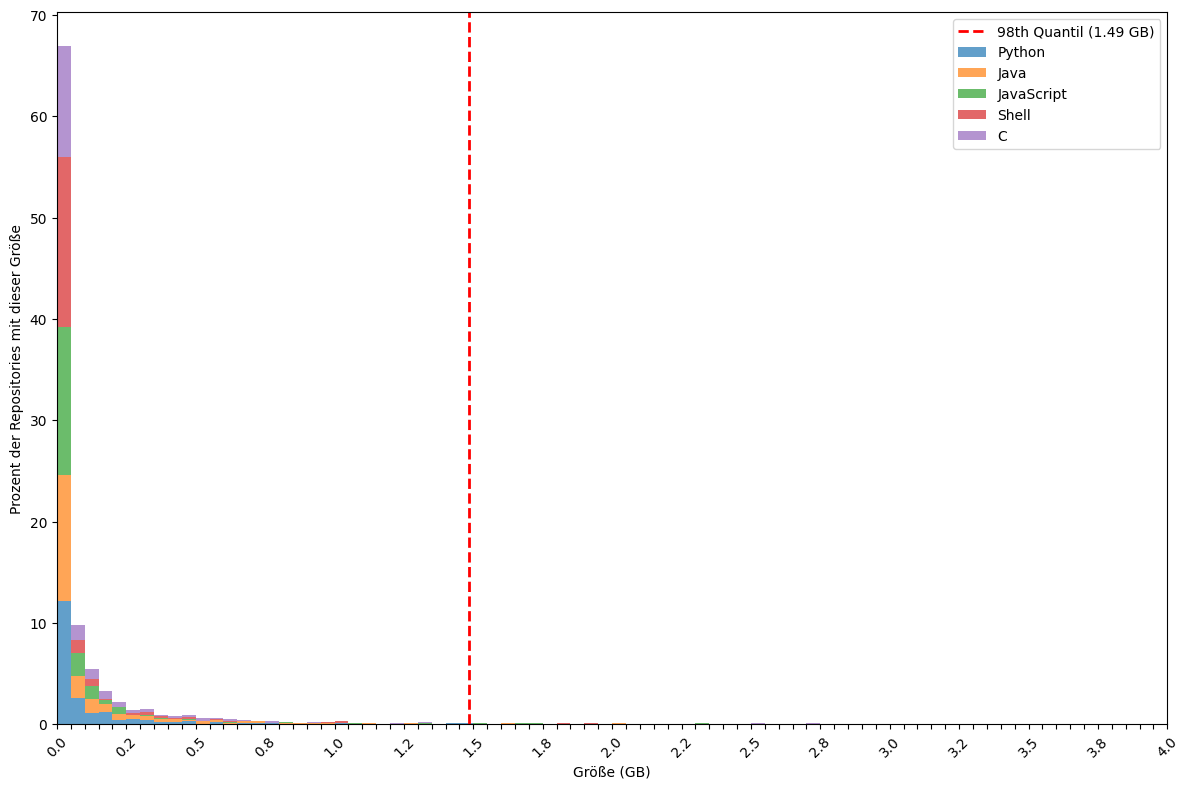
\includegraphics[width=0.8\textwidth]{images/datenanalyse/repoSizeUnfilteredVerteilung.png}
    \caption{Das Diagram zeigt, dass es deutlich mehr kleine Projekte gibt (logarithmisch abnehmend)}
    \label{fig:repoGroesseVerteilungUnfiltered}
\end{figure}

Man könnte argumentieren, warum macht ihr euch die arbeit und nehmt nicht einfach random Projekte? Weil wir spezifisch sicher gehen wollen projekte aller größen in einer linearen verteilung. ansonsten haben wir vorallem kleine Projekte, bei denen sowieso das treemap problem nicht so sehr auftritt, dann würden wir in den daten auch keine wirklichen änderungen sehen können (wahrscheinich) oder nicht so große. weil eher kleine projekte \ref{fig:cumSumRepoSizeLog}.

Deswegen wählen wir spezifisch Projekte bis zu 1,5GB (98er Quantil) aus. Wir wählen das so, dass wir eine lineare verteilung haben und ca. alle 0,1GB ein Projekt - also haben wir 15 Projekte pro Sprache -> 70 Projekte, die die grundlage für alle analysen und evals dieser ARbeit bieten. 
Zusätzlich gehen wir sicher, dass Projekte  wie \textit{The most comprehensive database of Chinese poetry} oder \textit{A list of funny and tricky JavaScript examples} nicht im datensatz enthalten sind, weil das keine echten Software-Applikationen sind, sondern sammlungen oder andere sachen, für die unsere Visualisierung nicht gedacht ist -> klar auch möglich natürlich, aber nich das Ziel dieser Arbeit.

In Abbildung \ref{fig:repoGroesseVerteilung} ist zu erkennen, dass wir relativ gleichmäßg die repos bis zu einer Größe von 1,5GB abdecken.  Die genau auswahl an repos ist in Anhang \ref{lst:selected_repos.json} zu finden.
\begin{figure}
    \centering
    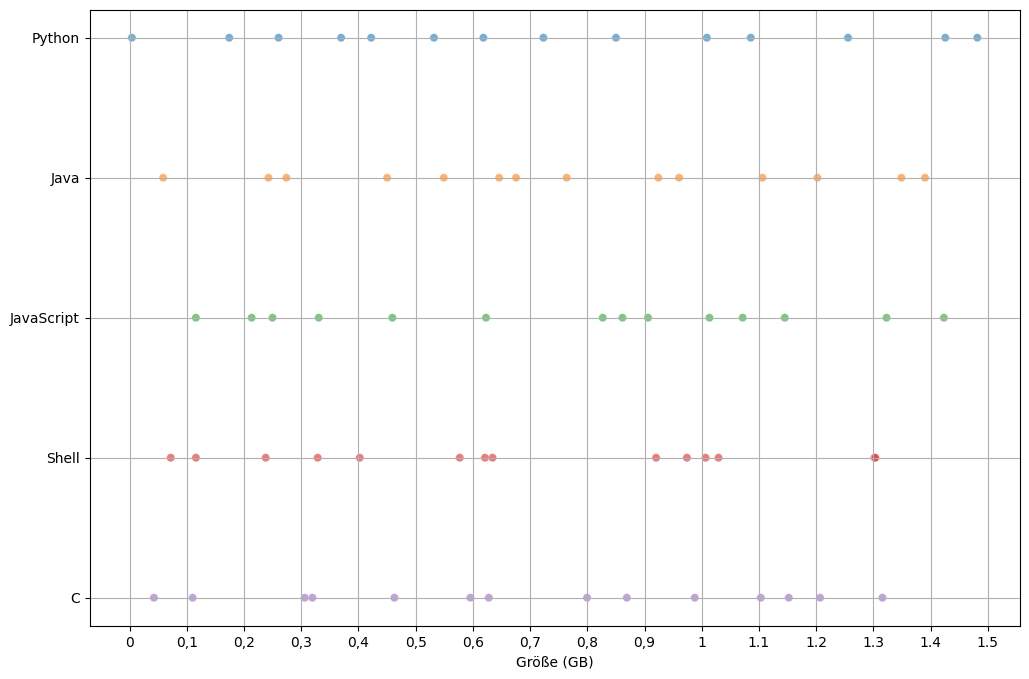
\includegraphics[width=0.8\textwidth]{images/datenanalyse/repoGrößeVerteilung.png}
    \caption{Die Verteilung der Projektgrößen der ausgewählten Repositories je Sprache.}
    \label{fig:repoGroesseVerteilung}
\end{figure}

Da die größe nicht 1 zu 1 mit der Anzahl an nodes korreliert. ein order zum beispiel nimmt fast keine größe ein. außerdem sind bei jeder sparche die dateien verschieden groß es gibt unterschiedliche anzahl an dateien die nicht betrachtet werden wie png, mp4 etc die zur größe aber nicth zur anzahl an nodes beitragen. Es ist zu erkennen, dass dadurch doch wieder mehr kleinenere Repos gibt, aber das akzeptieren wir einfach. \ref{fig:repoAnzahlNodesVerteilung} Besonders bei Shell ist zu erkennen, dass die Anzahl an Knoten nicht wirklich linear verteilt ist. Zeigt wie unterschiedlich die repos der verschiedenen Sprachen sind, trotzdem aktzeptieren wir das, am ende bildet es die Realität ab.

\begin{figure}
    \centering
    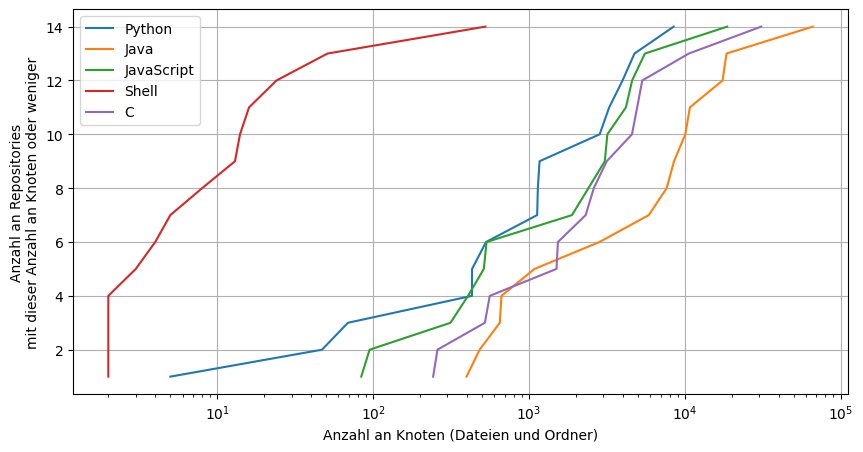
\includegraphics[width=0.8\textwidth]{images/datenanalyse/repoAnzahlNodesVerteilung.png}
    \caption{Die Verteilung der Anzahl an Knoten der ausgewählten Repositories je Sprache.}
    \label{fig:repoAnzahlNodesVerteilung}
\end{figure}

\subsection{Analyse der ausgewählten Repositories} \label{sec:analyseDerAusgewähltenRepositories}
Wie berechnen wir die Struktur der Repositories und wie bekommen wir metrik daten für diese REpos?
Wir clonen jedes repo und analysieren die Struktur der Repositories mit dem CodeCharta Analysis CLI Tools \cite{code_charta_wiki_ana}. Dieses Tool analysiert die Struktur der Repositories und berechnet für jede Datei (es werden nur Dateien betrachtet die zur entsprechenden Programmiersprache gehören, also zB. .py für Python) die Metriken, die wir später für die Visualisierung verwenden werden. Genutzt wird der unified parser mit diesem Command:
%ccsh unifiedparser "$name" -o "${REPOS_DIR}/${name}.cc.json" -nc "--verbose=false" "--exclude=" "--file-extensions="
Als ergebnis bekommen wir eine JSON-Datei, mit der in Abschnit \ref{sec:Problemstellung} definierten Struktur. Ein Beispiel ist auch im anhang (Listing \ref{lst:artificial.cc.json}) zu finden.

\section{Struktur von Softwareprojekten} \label{sec:strukturVonSoftwareprojekten}    

Im Abschnitt Problemstellung (Abschnit \ref{sec:Problemstellung}) wwurde das Format der Eingabe-Daten formal definiert (siehe Listing \ref{lst:nodeSchema}). Die Hierarschische-Struktur selbst ist offen in ihrer Größe und Form also zB. wie viele Kinder hat ein Knoten, wie Tief ist die Verschachtelung etc. Wir verscuhen das in diesem Kapitel einzuschreänken, also auf zu zeigen, wie hierarschiche strukturen, die aus software analyse auf file-basis laufen aussehen. UM nochmal klarer zu werden: die formale definition steht. aber in der praxis realität werden diese Strukturen aus der Datei-Hierachie von Software-Projekten entstehen. 

Warum wollen wir das tun? Weil wir uns erhoffen, erkenntnisse über die Datei-Struktur von Software-Projekten zu gewinnen, die uns helfen, die algorithmen genau für diese Strukturen zu optimieren und außerdem die Laufzeiten der algorithmen eine bessere einschätzung zu geben.

Im Grundlagen Kapitel wurde bereits erwähnt, dass die Metrik-Daten, die wir durch die Analyse von Code erhalten, spezielle Eigenschaften aufweist (siehe Abschnitt \ref{sec:SoftwareQualitaetsmetriken}). Diese Eigenschaften sind wichtig, um die Visualierung zu optimieren und zu wissen in welchem Rahmen sich die zu visualisierenden Daten bewegen. 

numberOfFiles: 3262.34 (avr), 708.50 (median), 7391.42 (std)
numberOfFolders: 958.76 (avr), 242.00 (median), 2089.59 (std)
numberOfNodes: 4221.10 (avr), 1108.50 (median), 9308.05 (std)